\begin{frame}
\centering
\textbf{Resultados para Nº Carathéodory}
\end{frame}

\section{Resultados Carathéodory}
\begin{frame}
\frametitle{Nº Carathéodory}
\framesubtitle{diâmetro 2}
\begin{columns}[T]
 \begin{column}{.5\textwidth}
\begin{proposition}
Considere $G$ um grafo de diâmetro 2 com vértice de corte, então $c(G) = 2$.
\end{proposition}
\begin{itemize}
    \item Um conjunto Carathéodory $S$ com $S\ge 3$ o vértice de corte não pode ser o parcial
    \item Os vértices de $S$ estão em componentes distintas
    \item O parcial está em componentes distintas de outros vértices de $S$ e não pode ser o vértice de corte
    \item O parcial não existe
\end{itemize}
\end{column}
\begin{column}{.5\textwidth}
\centering
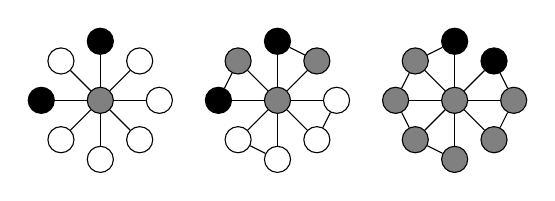
\begin{tikzpicture}[scale=0.5]
\node[circle,draw,fill=black!50] (v1) at (-13.5,-1) {};
\node[circle,draw,fill] (v3) at (-13.5,0.5) {};
\node[circle,draw,fill] (v9) at (-15,-1) {};
\node[circle,draw] (v7) at (-13.5,-2.5) {};
\node[circle,draw] (v5) at (-12,-1) {};
\node[circle,draw] (v8) at (-14.5,-2) {};
\node[circle,draw] (v6) at (-12.5,-2) {};
\node[circle,draw] (v4) at (-12.5,0) {};
\node[circle,draw] (v2) at (-14.5,0) {};
\draw  (v1) edge (v2);
\draw  (v1) edge (v3);
\draw  (v1) edge (v4);
\draw  (v1) edge (v5);
\draw  (v1) edge (v6);
\draw  (v7) edge (v1);
\draw  (v1) edge (v8);
\draw  (v1) edge (v9);

\node[circle,draw,fill=black!50] (v31) at (-9,-1) {};
\node[circle,draw,fill] (v33) at (-9,0.5) {};
\node[circle,draw,fill] (v39) at (-10.5,-1) {};
\node[circle,draw] (v37) at (-9,-2.5) {};
\node[circle,draw] (v35) at (-7.5,-1) {};
\node[circle,draw] (v38) at (-10,-2) {};
\node[circle,draw] (v36) at (-8,-2) {};
\node[circle,draw,fill=black!50] (v34) at (-8,0) {};
\node[circle,draw,fill=black!50] (v32) at (-10,0) {};
\draw  (v31) edge (v32);
\draw  (v31) edge (v33);
\draw  (v31) edge (v34);
\draw  (v31) edge (v35);
\draw  (v31) edge (v36);
\draw  (v37) edge (v31);
\draw  (v31) edge (v38);
\draw  (v31) edge (v39);

\node[circle,draw,fill=black!50] (v21) at (-4.5,-1) {};
\node[circle,draw,fill] (v23) at (-4.5,0.5) {};
\node[circle,draw,fill=black!50] (v29) at (-6,-1) {};
\node[circle,draw,fill=black!50] (v27) at (-4.5,-2.5) {};
\node[circle,draw,fill=black!50] (v25) at (-3,-1) {};
\node[circle,draw,fill=black!50] (v28) at (-5.5,-2) {};
\node[circle,draw,fill=black!50] (v26) at (-3.5,-2) {};
\node[circle,draw,fill] (v24) at (-3.5,0) {};
\node[circle,draw,fill=black!50] (v22) at (-5.5,0) {};
\draw  (v21) edge (v22);
\draw  (v21) edge (v23);
\draw  (v21) edge (v24);
\draw  (v21) edge (v25);
\draw  (v21) edge (v26);
\draw  (v27) edge (v21);
\draw  (v21) edge (v28);
\draw  (v21) edge (v29);
\draw  (v24) edge (v25);
\draw  (v26) edge (v25);
\draw  (v28) edge (v29);
\draw  (v28) edge (v27);
\draw  (v22) edge (v29);
\draw  (v23) edge (v22);

\draw  (v34) edge (v33);
\draw  (v36) edge (v35);
\draw  (v37) edge (v38);
\draw  (v39) edge (v32);
\end{tikzpicture}
\end{column}
\end{columns}
\end{frame}

\begin{frame}
\frametitle{Nº Carathéodory}
\framesubtitle{diâmetro 2}
\begin{columns}[T]
\begin{column}{.4\textwidth}
\begin{coro}
    Seja $G$ um grafo MST $C_5[p,q,r,s,t]$ e $|p|$, $|q|$, $|r|$, $|s|$ e $|t|$ for maior que 1 então $c(G) = 2$.
\end{coro}
\begin{itemize}
    \item Um conjunto Carathéodory $S$ com $S\ge 3$ contem 2 ou mais vértices não adjacentes
    \item Qualquer 2 vértices não adjacentes são um conjunto envoltório
    \item $\not \exists S^\prime \subset S$ tal que $S^\prime$ é envoltório
\end{itemize}
\end{column}
\begin{column}{.6\textwidth}
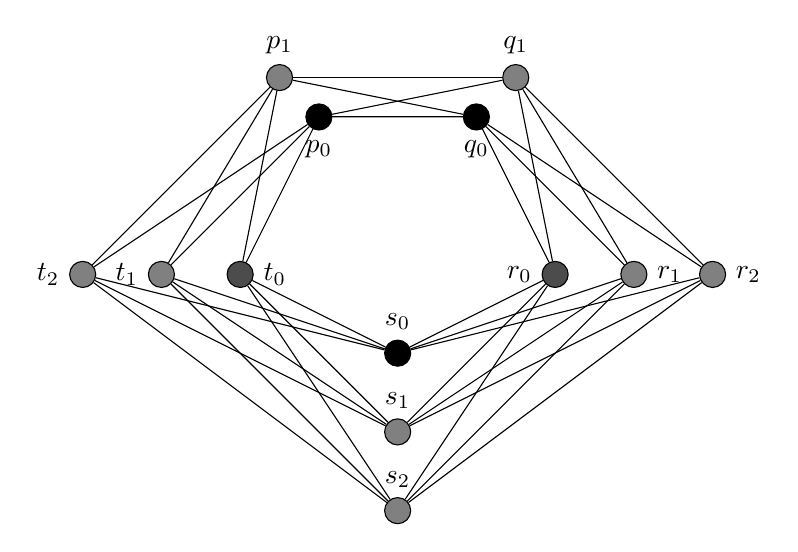
\begin{tikzpicture}
\node[draw,circle,label=$s_0$,fill] (v4) at (-1,-4) {};
\node[circle,draw,label=right:$t_0$,fill=black!70] (v5) at (-3,-3) {};
\node[circle,draw,label=below:$p_0$,fill] (v1) at (-2,-1) {};
\node[circle,draw,label=below:$q_0$,fill] (v2) at (0,-1) {};
\node[draw,circle,label=left:$r_0$,fill=black!70] (v3) at (1,-3) {};
\draw (v1) -- (v2) -- (v3) -- (v4) -- (v5) -- (v1);
\node[draw,circle,label=$p_1$,fill=black!50] (v6) at (-2.5,-0.5) {};
\node[draw,circle,label=$q_1$,fill=black!50] (v9) at (0.5,-0.5) {};
\node[draw,circle,label=$s_1$,fill=black!50] (v13) at (-1,-5) {};
\node[draw,circle,label=$s_2$,fill=black!50] (v12) at (-1,-6) {};
\node[draw,circle,label=right:$r_1$,fill=black!50] (v15) at (2,-3) {};
\node[draw,circle,label=right:$r_2$,fill=black!50] (v14) at (3,-3) {};
\node[draw,circle,label=left:$t_1$,fill=black!50] (v8) at (-4,-3) {};
\node[draw,circle,label=left:$t_2$,fill=black!50] (v7) at (-5,-3) {};
	
\draw  (v6) edge (v7);
\draw  (v6) edge (v8);
\draw  (v6) edge (v5);
\draw  (v6) edge (v9);
\draw  (v6) edge (v2);
\draw  (v12) edge (v7);
\draw  (v13) edge (v7);
\draw  (v8) edge (v4);
\draw  (v4) edge (v7);
\draw  (v8) edge (v13);
\draw  (v8) edge (v12);
\draw  (v14) edge (v12);
\draw  (v14) edge (v13);
\draw  (v14) edge (v4);
\draw  (v15) edge (v4);
\draw  (v13) edge (v15);
\draw  (v12) edge (v15);
\draw  (v9) edge (v3);
\draw  (v9) edge (v15);
\draw  (v14) edge (v9);
\draw  (v1) edge (v9);
\draw  (v1) edge (v7);
\draw  (v1) edge (v2);
\draw  (v14) edge (v2);
\draw  (v1) edge (v8);
\draw  (v2) edge (v15);
\draw  (v3) edge (v13);
\draw  (v13) edge (v5);
\draw  (v3) edge (v12);
\draw  (v12) edge (v5);
\end{tikzpicture}
\end{column}
\end{columns}
\end{frame}

